
\section{Method} 
\label{sec:method}
\vspace{-2mm}
The inputs to our method are a base mesh $\basemesh = (\baseverts, \basefaces)$ (e.g., a bust, as shown in \autoref{fig:main_method}) and an object or accessory mesh $\objectmesh = (\objectverts, \objectfaces)$ (e.g., a hat) in arbitrary relative position, together with a highlighted region of the base mesh $\highlightedmesh \subseteq \basemesh$ (the orange region in \autoref{fig:main_method}) and an optional text string describing both shapes.
The algorithm we will detail in this section will output a transformed object mesh $\transformation (\objectmesh) = (\transformation (\objectverts), \objectfaces)$ that can be superimposed with the base mesh \emph{tightly}, in a \emph{semantically and physically realistic} way \emph{without intersections}.

\begin{figure*}[t]
    \centering
    \vspace{3mm}
    %\vspace{-2cm}
    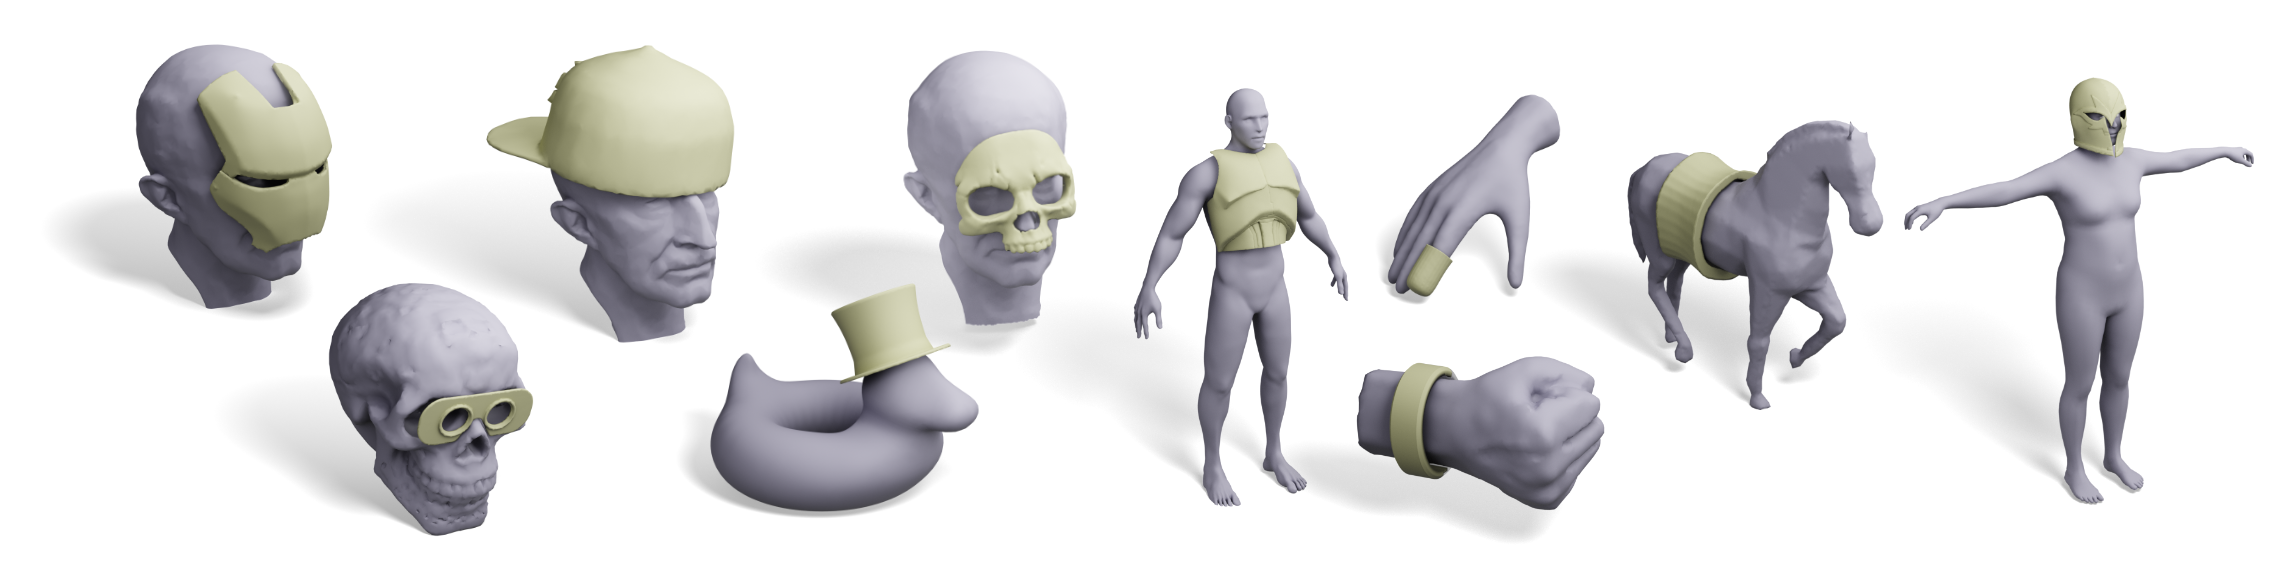
\includegraphics[width=\textwidth]{figures/gallery/gallery.png}
    \captionof{figure}{\ourmethod{} is capable of fitting a wide variety of accessories on a range of different meshes. Our method handles challenging spatial relationships such as sliding glasses along a head to align with the ears, positioning hats and helmets to conform to head curvature, wrapping bands around articulated limbs, and fitting objects along long, curved surfaces. These examples demonstrate the flexibility of our fitting trajectory and its ability to adapt accessories to widely varying shapes and poses.}
    %\vspace{-2cm}
    \label{fig:gallery}
    \vspace{-3mm}
\end{figure*}%


These goals often act in opposition to one another; for example, achieving a tighter fit will often produce intersections, while removing intersections will tend to produce a looser fit.
We address this challenge through a multi-step optimization framework in which the different constraints, objectives and degrees of freedom of the problem are introduced one at a time.
From an initial (scaled) rigid transformation $\rigid_0$ (we defer discussion of initialization strategies to \autoref{sec:initialization}), we begin by rigidly and tightly fitting the object onto the base mesh, potentially \emph{with} intersections (see $\rigid_1$ in \autoref{sec:step1}).
Then, we simulate possible rigid object attachment trajectories using physically-inspired losses to obtain a loose \emph{non-intersecting} configuration $\rigid_2$ (see \autoref{sec:step2}), which we then refine, first into a tight rigid non-intersecting fit $\rigid_3$ (see \autoref{sec:step3}) and then through a diffusion-guided deformation (see \autoref{sec:step4}) to produce our final transformation $\transformation$.


\subsection{Step 1: Tight fit with intersections}
\label{sec:step1}



We will represent the space of all possible scaled rigid transformations through rotation, translation and scale parameters $\rigid(\parameters) = \rigid (\rotation, \translation, \scale)$, where $\rotation$ are the standard continuous 6D representation of 3D rotations \cite{zhou2019continuity}.
To find a rigid transformation that aligns the object mesh with the highlighted region of the base mesh (potentially while intersecting with it), one could naively optimize the two-sided vertex-to-mesh total distance between the base and (highlighted) object meshes
\begin{equation*}
    \sum_{\vertex_{i} \in \objectmesh} d (\rigid(\parameters)\vertex_i, \highlightedmesh)^2 +  \sum_{\vertex_{j} \in \highlightedmesh} d(\vertex_j, \rigid (\parameters)\objectmesh)^2\, .
\end{equation*}
Optimizing such energy directly would present two key challenges. First, the quadratic computational complexity would place a severe limit on mesh size. Secondly, the dense computational graph would present storage and performance issues during GPU autodifferentiation.



We fix the first of these problems through a Bounding Volume Hierarchy tailor-made to exploit vectorized operations in the GPU.
We build our BVH in a similar way to a traditional Axis-Aligned Bounding Box hierarchy (see \cite{shirley2009fundamentals}, Chap. 12). However, we abort any top-down traversal when a box contains fewer than $K$ mesh triangles, resorting instead to a tensorized batch query in the GPU (in our experiments, we fix $K=1,000$).

To avoid overhead from dense computational graphs, and to make our algorithm robust to haphazardly defined contact regions, we introduce a \emph{masked} distance function $\hat{d}$ that is identical to the true distance $d$ but which zeroes out any entry above a threshold $\thresholdprox$ (in our experiments, $\thresholdprox=0.5$). This lets us define our \emph{proximity loss}
\begin{equation*}
    \mathcal{L}_{p}(\parameters) = \sum_{\vertex_{i} \in \objectmesh} \hat{d} (\rigid(\parameters)\vertex_i, \highlightedmesh)^2 +  \sum_{\vertex_{j} \in \highlightedmesh} \hat{d}(\vertex_j, \rigid (\parameters)\objectmesh)^2\, ,
\end{equation*}
which we optimize to find $\parameters^\star$ and, with it, our first scaled rigid transformation $\rigid_1 = \rigid (\parameters^\star)$ (see \autoref{fig:main_method}).




\subsection{Step 2: Trajectory-based intersection solve}
\label{sec:step2}

In the previous step, we rigidly transformed the object to tightly fit into the base mesh; however, this often introduces intersections between them (see \autoref{fig:trajectory_method}). We will now turn this intersecting configuration into a non-intersecting one, without compromising too much on tightness.


To do so, we will draw inspiration from how one puts on an accessory: for most tightly-fitting ones, there exists a valid, intersection-free trajectory that moves the object from a detached configuration into a tight fit with the base mesh (e.g., the process of putting on a hat or a ring).

We will begin by generating a large number of potential starting points for this trajectory, as shown in \autoref{fig:trajectory_method}. To do so, we draw rigid transformation's parameters from independent Gaussian and uniform distributions
\begin{align*}
\mathbf{e}_i \sim \gaussian (0,\sigma_{rot})\,,&\quad \scale \sim \uniform(\scale_{\min}, \scale_{\max})\,,\\
\translation_{\perp} \sim \gaussian (0,\sigma_{\perp})\,,&\quad \translation_{\parallel} \sim \gaussian (\mu_{\parallel},\sigma_{\parallel})
\end{align*}
where we have separated $\translation$ into the components orthogonal ($\translation_{\perp}$) and parallel ($\translation_{\parallel}$) to the average normal in the base mesh's highlighted region $\highlightednormal$ (see \autoref{fig:trajectory_method}, left). We draw samples from these distributions to produce candidate scaled rigid transformations $\rigid$ and check whether $\rigid \objectmesh$ intersects with the base mesh $\basemesh$, repeating this sampling process and progressively increasing the values of $\sigma_{rot}$ and $\sigma_{\parallel}$ until we find $\numnonintersecting$ non-intersecting candidate transforms $\rigid^1,\dots,\rigid^{\numnonintersecting}$ (in our experiments, $\numnonintersecting = 100$).

\begin{wrapfigure}[9]{r}{0.55\linewidth}
    \centering
    \vspace{-6mm}
    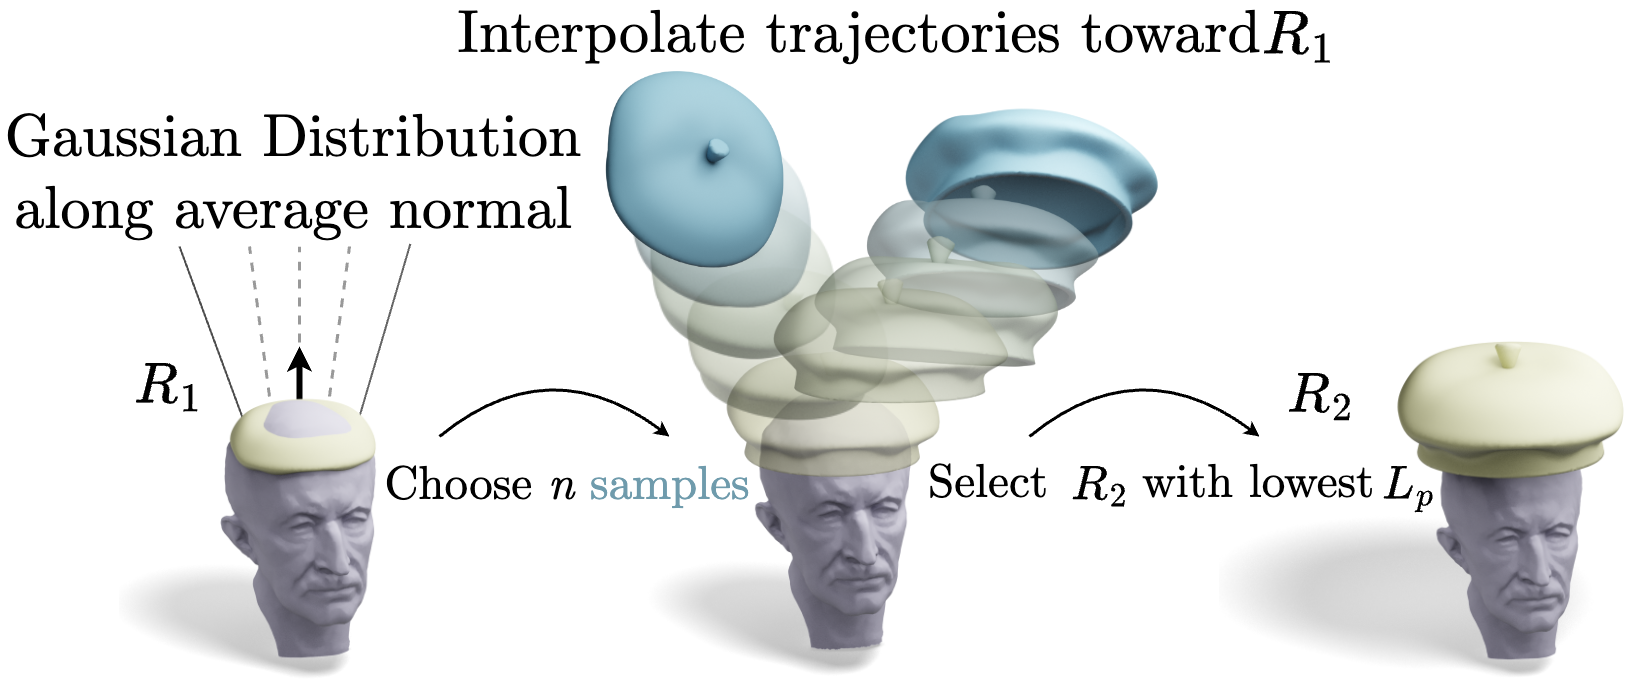
\includegraphics[width=\linewidth]{figures/trajectory_method/trajectory_method.png}
    \caption{}
    % \caption{To find a non-intersecting configuration, we simulate several possible object trajectories and sample different timesteps (see \autoref{sec:step2}). Among all non-intersecting candidates, we select the one closest to the target region of the base mesh.}
    \label{fig:trajectory_method}
\end{wrapfigure}

Once $\rigid^1,\dots,\rigid^{\numnonintersecting}$ have been identified, we use spherical linear interpolation (SLERP) to build candidate trajectories from each non-intersecting $\rigid^i$ to the intersecting transformation from the previous step $\rigid_1$ (see \autoref{fig:trajectory_method}, transparent frames). We sample $\numtimesteps$ discrete timesteps of each trajectory, keeping only the non-intersecting ones (in our experiments, $m=25$). After gathering all non-intersecting timesteps for all candidate trajectories $R^i$, we make $\rigid_2$ be the transformation with the lowest proximity loss $\mathcal{L}_{p}$ (\autoref{fig:trajectory_method}, right).

\begin{figure*}[t]
    \centering
    \vspace{3mm}
    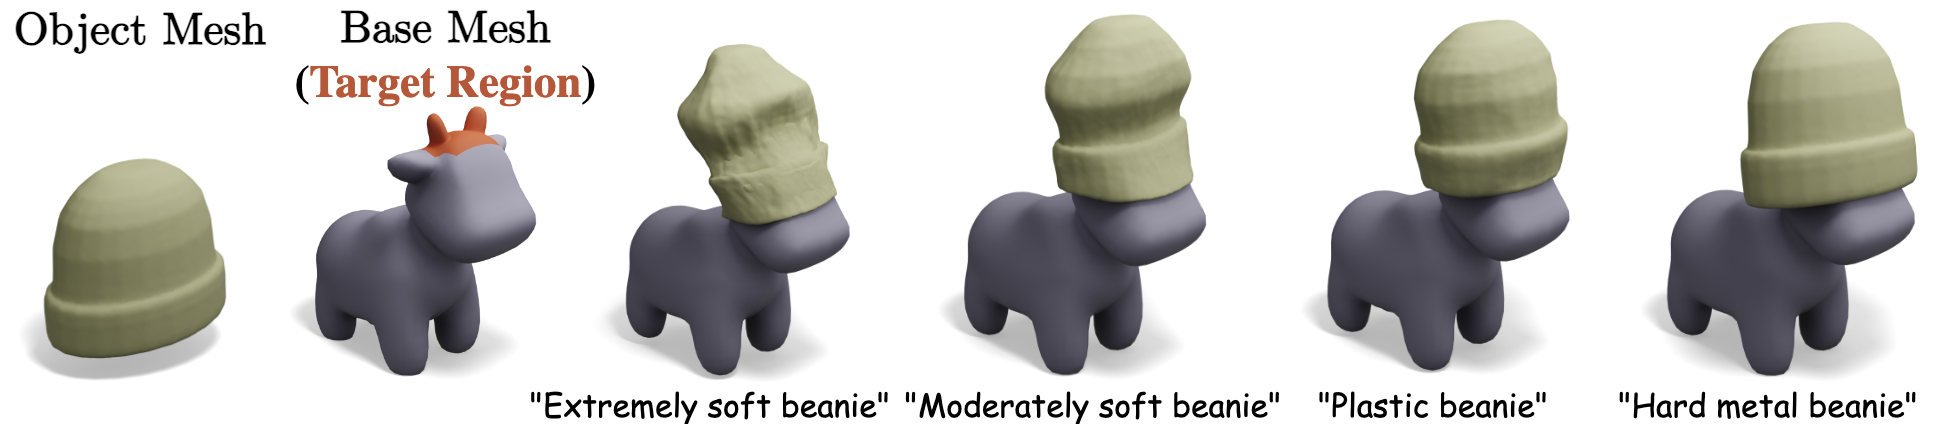
\includegraphics[width=\textwidth]{figures/materials/materials.png}
    \captionof{figure}{\ourmethod{} is capable of fitting the accessory onto the base mesh in a way that considers material properties. Instead of having to specify the numeric material parameters, artists can provide material guidance through text prompts, that get combined with rendered images and interpreted by a VLM to output specific elastic parameters.}
    %\vspace{-2cm}
    \label{fig:materials}
\end{figure*}%





\subsection{Step 3: Rigid finetuning}
\label{sec:step3}
The output of the previous section is a (scaled) rigid transformation $\rigid_2$ that moves the accessory reasonably close to the highlighted region of the base mesh without intersecting it; however, it likely fits too loosely to seem realistic (see \autoref{fig:main_method}, middle).

To refine this transformation, we draw inspiration from works in the physically-based simulation area, in which the relative positions of many objects are often assumed to minimize some physically meaningful energy (e.g., gravity) subject to non-intersecting constraints.
A common strategy for imposing these constraints is by adding repulsive energy terms to the optimization \cite{baraff1998large,li2020incremental,lan2024efficient}.
In a similar way, starting from $\rigid_2 = \rigid(\parameters_2)$, we will optimize the loss
\begin{equation}\label{equ:total-loss}
\mathcal{L}(\parameters) = \mathcal{L}_{p}(\parameters) + \mathcal{L}_{\text{IPC}}(\parameters)\,,
\end{equation}
where $\mathcal{L}_{p}$ is the proximity loss introduced in \autoref{sec:step1} and $\mathcal{L}_{\text{IPC}}$ is the \emph{Incremental Potential Contact} barrier energy \cite{li2020incremental}, given by
\begin{equation*}
\mathcal{L}_{\text{IPC}}(\parameters) = \sum_{\vertex_i \in \objectmesh} b_{\contactthreshold}\left(d\left(\rigid(\parameters)\vertex_i,\basemesh\right)\right)\,,
\label{contact_loss}
\end{equation*}
where
\begin{equation*}
    b_h(x) =
    \begin{cases}
      -(x-h)^{2}\ln\left( \dfrac{x}{h} \right) & \text{if}\quad x < h \\
      0       & \text{otherwise.}
    \end{cases}
\end{equation*}
This energy penalizes the object's vertices as they approach the base surface, with a second-order continuous (\( C^2 \)) form at the boundary \( d\left(\rigid(\parameters)\vertex_i,\basemesh\right) = \contactthreshold \), and naturally vanishes as \( d\left(\rigid(\parameters)\vertex_i,\basemesh\right) \to \contactthreshold \) or beyond (in our experiments, $h=0.01$). In addition to its use as an optimization energy in this section, we also use $\mathcal{L}_{\text{IPC}}$ to classify if a configuration is or not intersecting in the previous sections.

Minimizing the total loss from \autoref{equ:total-loss} using gradient-based optimization, starting from $\rigid_2$, results in a novel (scaled) rigid transformation $\rigid_3 = \rigid(\parameters^\star)$ that fits the object tightly without intersections over the base mesh.



\begin{figure*}[t]
\vspace{3mm}
\centering
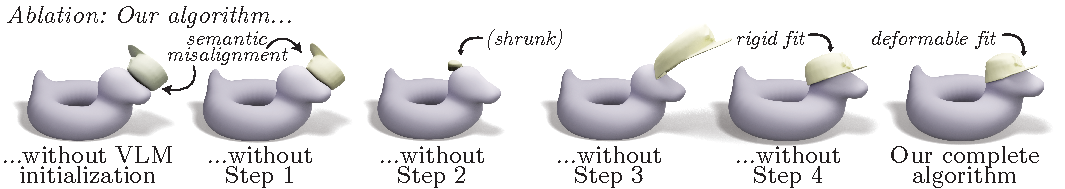
\includegraphics[width=\textwidth]{figures/placeholders/steps-ablation.pdf}
\caption{\ourmethod{} uses a multi-step process, where each of them is critical for achieving a desirable mesh to mesh composition result. Omitting any of the steps yields a semantically (two left results) or physically (two center results) unplausible solutions. Utilizing Step 4 further improves the result (second from the right), allowing the asset to deform and better fit the base mesh (rightmost).} %\rana{something more about what }
\label{fig:steps-ablation}
\end{figure*}



\subsection{Step 4: Elastic deformation}
\label{sec:step4}

The physically-inspired optimization of the previous step outputs a rigidly transformed mesh $\restmesh = \rigid_3 (\objectmesh) = ( \rigid_3 (\objectverts), \objectfaces)$, which we interpret as the best possible \emph{rigid fit} of the object onto the base mesh.
In reality, however, many accessories fit their wearer more tightly by undergoing small deformations: a hat is stretched by a head's shape, a necklace drapes over a person's chest, a face mask deforms to fit the nose and mouth of a surgeon.
Beyond physical deformation, an artist may also wish to perform small physical non-rigid edits on a general-purpose object mesh to better match their specific creative intentions.

To model this final fit, we will follow the lead of prior work \cite{aigerman2022neural, kim2025meshup, gao2023textdeformer, dinh2025geometry} and parametrize the object mesh deformation via a per-face Jacobian field \( \{J_i \in \mathbb{R}^{3 \times 3}\} \), which describes the local transformation of the surface. From these Jacobians, one can recover vertex-wise deformations $ \vertext_i = \transformation (\vertex_i) $  through a Poisson-like least-squares minimization:
\begin{equation}\label{equ:poisson}
\transformation^\star = \arg\min_t \sum_i a_i \left\| \nabla_i(t) - J_i \right\|_2^2\, ,
\end{equation}
where $a_i$ is the area of the $i$-th triangle in the mesh. This allows us to write $\transformation$ as a function of the per-face Jacobians $\transformation = \transformation(J_1, J_2, \dots) = \transformation(\{J_i\})$.
Our proximity and IPC losses from the previous section can thus be analogously defined for this non-rigid setting as
\begin{align}
\mathcal{L}_{p}(\{J_i\}) & = \sum_{\vertex_{i} \in \objectmesh} \hat{d} (\transformation(\{J_i\})\vertex_i, \highlightedmesh)^2  
+  \sum_{\vertex_{j} \in \highlightedmesh} \hat{d}(\vertex_j, \transformation(\{J_i\})\objectmesh)^2\,
\end{align}
and
\begin{align}
\mathcal{L}_{\text{IPC}}(\{J_i\}) & = \sum_{\vertex_i \in \objectmesh} b_{\contactthreshold}\left(d\left(\transformation(\{J_i\})\vertex_i,\basemesh\right)\right)\,,
\end{align}
where we use a lower proximity threshold value of $\ell=0.01$ to zero out distance entries, enforcing the deformation to be conservatively confined to its local boundries. 
The point-to-mesh distances $d$ are once again computed using a bounding volume hierarchy; however, this hierarchy is recomputed every $20$ iterations due to the presence of deformations.
Additionally, we follow the strategy proposed by \emph{MeshUp} \cite{kim2025meshup} and guide the deformation towards a semantically meaningful fit via Score Distillation Sampling (SDS).
Let \( z \) denote a rendered image of the current mesh, and \( \mathcal{T} \) a guiding text prompt. At each iteration, we sample a timestep \( t \sim \mathcal{U}(0,1) \) and a noise vector \( \epsilon \sim \mathcal{N}(0,I) \), and use the gradient
$$
\nabla_{J_i} \mathcal{L}_{\text{SDS}}(\{J_i\}) = w(t)\left(
\epsilon_\omega(z_t, \transformation(\{J_i\}), t) - \epsilon
\right)
\cdot
\frac{\partial z_t}{\partial J_i}.
$$
Finally, some deformations are more physically realistic than others, and different materials will deform by different amounts. To model this, we include the standard elastic NeoHookean energy as a loss term (see \cite{sifakis2012fem}, Chap. 3.6),
\begin{align*}
\mathcal{L}_e (\{J_i\}) = & \sum_i \left(\frac{\mu}{2}\left(\tr(J_i^\top J_i) - 3\right)\right.
- \left.\mu \log(\det(J_i))
 + \frac{\lambda}{2} \log^2(\det(J_i)) \right)
\end{align*}
where the material parameters $\lambda$ and $\mu$ are either given as input to our algorithm or inferred either from rendered images or text descriptions by our multi-agent initialization framework (see \autoref{sec:initialization}).
We end by minimizing the total loss
\[
\mathcal{L} = \mathcal{L}_{p} + \mathcal{L}_{\text{IPC}} + \lambda_{\text{SDS}} \mathcal{L}_{\text{SDS}} + \lambda_{e} \mathcal{L}_e\, ,
\]
with respect to $\{J_i\}$ using gradient-based optimization, and solve \autoref{equ:poisson} to obtain our final transformation $\transformation$ (see \autoref{fig:main_method}, right). As desired, $\transformation$ fits the object mesh tightly onto the base mesh in a semantically and physically realistic way without intersections, ending our algorithm.





\subsection{Initialization}
\label{sec:initialization}
Like any gradient-based optimization, our algorithm is sensitive to initialization; in particular, it depends on the initial relative configuration of the two meshes that is then modified in steps one through four.
Experimentally, we find that our method is relatively robust to different initial configurations; however, the most adversarial of them can cause it to converge to undesirable local minima (see \autoref{fig:initialization}).

To avoid these, we initialize the relative configuration using a VLM.  First, from a text description (e.g., "a hat") and renderings of the object, the VLM is prompted to produce a canonical reference frame for it (e.g., "the front of the hat is the region with a visor, the top part of the hat...."). This process is repeated for the base mesh. Then, several different random orientations are sampled for the object mesh. For each, a VLM is used to deduce its alignment with the canonical reference frame and with the base mesh's. The latter is used to score each configuration, and we select the highest-scoring one as initialization (see Supplementary Material for details). 


 An additional agent uses user input text to output the the material parameters $\lambda, \mu$, giving users a fully-integrated, text-based control over the entire optimization process (see \autoref{fig:main_method}).
More details about our initialization scheme are provided in the Supplementary.
